\section{The Two-Level System\footnote{cf. \cite{cohen}, chapter 4}}

		There are many examples for two-level systems that can be found in nature:
		\begin{itemize}
			\item Spin of the electron: Up vs. down state
			\item Two-level atom with one electron (simplified): Excited vs. ground state
			\item Structures of molecules, e.g., \hyperref[fig:twostate]{NH\textsubscript{3}}
		\end{itemize}
		Two-level systems are also used excessively in information technology.
		How do we induce dynamics, i.e., population transfer between the two levels $\ket{1}$ and $\ket{2}$? The time evolution is merely
		\begin{align}
			a_1\ket{1}\exp{-i{E_1 t}/{\hbar}} + a_2\ket{2}\exp{-i{E_2 t}/{\hbar}},
		\end{align}
		so that the occupation probabilities stay the same. 
		
		So far, we described the system in an eigenbasis of the Hamiltonian.
		If we choose a Hamiltonian which is not diagonal in the basis of interest, we will get a transfer of population between the two states.

				\paragraph{Example.}
					\begin{align}
						H=\frac{\hbar}{2}\Omega_x(\ket{2}\bra{1} + \ket{1}\bra{2}),
					\end{align}
					where $\Omega_x$ is the Rabi frequency.

				\paragraph{Note.} Sometimes it can be helpful to work in the Heisenberg picture, where the time evolution is added to the operators describing observables rather than state kets:

					\begin{align}
						\hat{A}_H=\eexp{i{\hat{H} t}/{\hbar}} \hat{A}_S \eexp{-i{\hat{H} t}/{\hbar}}
					\end{align}
					where $\eexp{-i{\hat{H} t}/{\hbar}}$ is a time evolution operator (N.B.: $\hat{H}_S = \hat{H}_H$). The time evolution of $\hat{A}_H$ is:
					\begin{align}
						\notag \diff{}{t} \hat{A}_H &=&& \frac{i}{\hbar}\hat{H}\eexp{i{\hat{H}t}/{\hbar}}\hat{A}_S \eexp{-i{\hat{H} t}/{\hbar}}\\ 
						&&-&\frac{i}{\hbar} \eexp{i{\hat{H} t}/{\hbar}}\hat{A}_S \eexp{-i{\hat{H}t}/{\hbar}}\hat{H}+\diffp{\hat{A}_H}{t}\\
						&=&& \frac{i}{\hbar}\left[\hat{H},\hat{A}_H\right] + \eexp{i{\hat{H}t}/{\hbar}}\diffp{\hat{A}_S}{t}\eexp{-i{\hat{H}t}/{\hbar}}
					\end{align}

					In the Heisenberg picture the state vectors are time-in\-de\-pen\-dent:
					\begin{align}
						\ket{\psi}_H \equiv \ket{\psi(t=0)}=\eexp{i{\hat{H}}t/{\hbar}} \ket{\psi(t)}.
					\end{align}
					Therefore, the results of measurements are the same in both pictures:
					\begin{align}
						\bra{\psi(t)}\hat{A}\ket{\psi(t)} = \bra{\psi}_H \hat{A}_H \ket{\psi}_H.
					\end{align}
					For example, applying this to the spin operators yields:
					\begin{align}
						\diff{}{t}\hat{s}_{i,H}=\frac{i}{\hbar}\left[\hat{H},\hat{s}_{i,H}\right].
					\end{align}

		\subsection{Hamiltonian, Eigenstates and Matrix Notation}

			We consider two eigenstates $\ket{\varphi_1}$, $\ket{\varphi_2}$ of the Hamiltonian $\hat{H}_0$ with
			\begin{align}
				\hat{H}_0\ket{\varphi_1}=E_1\ket{\varphi_1}, \qquad \hat{H}_0\ket{\varphi_2}=E_2\ket{\varphi_2}.
			\end{align}
			The eigenstates can be expressed in matrix notation:
			\begin{align}
				\ket{\varphi_1}=\left( \begin{array}{c} 1 \\ 0 \end{array} \right), \qquad \ket{\varphi_2}=\left( \begin{array}{c} 0 \\ 1 \end{array} \right),
			\end{align}
			so that $\hat{H}_0$ be written as a diagonal matrix
			\begin{align}
				\hat{H}_0 = \left(\begin{array}{cc} E_1 & 0 \\ 0 & E_2 \end{array}\right).
			\end{align}
			Any arbitrary state 
			\begin{align}
				\ket{\phi} = \left( \begin{array}{c} c_1 \\ c_2 \end{array} \right) = \left( \begin{array}{c} \braket{\varphi_1|\phi} \\ \braket{\varphi_2|\phi} \end{array} \right)
			\end{align}
			can be expressed in terms of the eigenstates of the Hamiltonian:
			\begin{align}
				\ket{\phi} = \sum_i c_i \ket{\varphi_i}.
			\end{align}
			If we apply $\hat{H}_0$ to the arbitrary state, we get:

			\begin{align}
				\ket{\phi'} &=\hat{H}_0 \ket{\phi}\\ 
				&= \sum\limits_{i,j} \ket{\varphi_i}\bra{\varphi_i} \hat{H}_0 \ket{\varphi_j}\braket{\varphi_j|\phi}\\
				&= \sum\limits_i \ket{\varphi_i} \overbrace{\sum\limits_j  \underbrace{\bra{\varphi_i} \hat{H}_0 \ket{\varphi_j} }_{H_{ij}}  \braket{\varphi_j|\phi}}^{c_i'}\\
				&= \sum_i c_i' \ket{\varphi_i}
			\end{align}
			% &= \sum\limits_i \ket{\varphi_i}  \sum\limits_j  \bra{\varphi_i} \hat{H}_0 \ket{\varphi_j}  \braket{\varphi_j|\phi}\\
			% &= \sum\limits_i \ket{\varphi_i} \sum\limits_j  \underbrace{\bra{\varphi_i} \hat{H}_0 \ket{\varphi_j} }_{H_{ij}}  \braket{\varphi_j|\phi}\\
			% &= \sum\limits_i \ket{\varphi_i} \overunderbraces{&&\br{1}{H_{ij}}}{& {\sum\limits_j} & \bra{\varphi_i} \hat{H}_0 \ket{\varphi_j} & \braket{\varphi_j|\phi}}{&\br{3}{c_i'}}\\
			We can also use matrix notation to express $\ket{\phi'}$:
			\begin{align}
				\left( \begin{array}{cc} \bra{\varphi_1}\hat{H}_0\ket{\varphi_1} & \bra{\varphi_1}\hat{H}_0\ket{\varphi_2} \\ \bra{\varphi_2}\hat{H}_0\ket{\varphi_1} & \bra{\varphi_2}\hat{H}_0\ket{\varphi_2} \end{array} \right)\left( \begin{array}{c} \braket{\varphi_1 | \phi} \\ \braket{\varphi_2|\phi} \end{array} \right).
			\end{align}

		\subsection{External Perturbation $\hat{W}$}

			We obtain the perturbed Hamiltonian $\hat{H}$ by adding a small, external perturbation  $\hat{W}$ to the unperturbed Hamiltonian:
			\begin{align} \label{eq:perturbedhamiltonian}
				\hat{H} = \hat{H}_0 + \hat{W}.
			\end{align}
			The eigenstates of the perturbed Hamiltonian will then be:
			\begin{align}
				\hat{H}\ket{\psi_{\pm}}=E_\pm \ket{\psi_\pm}.
			\end{align}

		\subsection{Static Properties}

			In the unperturbed basis $\left\{\ket{\varphi_1},\ket{\varphi_2}\right\}$ we get

			\begin{align}
				\hat{H} = \left(\begin{array}{cc} \tilde{E_1} & W_{12} \\ W^*_{12} & \tilde{E_2}\end{array}\right) \quad \text{with} \quad \tilde{E_i} = E_i + W_{ii}
			\end{align}
			for the perturbed Hamiltonian. Diagonalizing this Hermitian matrix yields
			\begin{align}\label{eq:Epm}
				E_\pm = \frac{1}{2}\left(\tilde{E_1}+\tilde{E_2}\right) \pm \frac{1}{2} \sqrt{\left(\tilde{E}_1-\tilde{E}_2\right)^2+4 \left|W_{12}\right|^2}
			\end{align}
			for the eigenenergies. The corresponding eigenvectors are:
			\begin{align}
				\ket{\psi_+}&=&\hspace{-2mm}&\cos\left(\frac{\theta}{2}\right) \eexp{-i{\varphi}/{2}}\ket{\varphi_1}+\sin\left(\frac{\theta}{2}\right) \eexp{i{\varphi}/{2}}\ket{\varphi_2}, \label{eq:staticpsiplus} \\ 
				\ket{\psi_-}&=&\hspace{-2mm}-&\sin\left(\frac{\theta}{2}\right) \eexp{-i{\varphi}/{2}}\ket{\varphi_1}+\cos\left(\frac{\theta}{2}\right) \eexp{i{\varphi}/{2}}\ket{\varphi_2}, \label{eq:staticpsiminus}
			\end{align}
			where 
			\begin{align} \label{eq:parameters}
				\tan(\theta) = \frac{2|W_{12}|}{\tilde{E}_1-\tilde{E}_2} \quad \text{and} \quad W_{12} \equiv |W_{12}|\cdot \eexp{-i\varphi}.
			\end{align}
			For the further discussion we define:
			\begin{align}
				E_m \coloneqq \frac{1}{2}\left(\tilde{E}_1+\tilde{E}_2\right),\\
				\Delta \coloneqq \frac{1}{2}\left(\tilde{E}_1-\tilde{E}_2\right),
			\end{align}
			so that \eqref{eq:Epm} becomes:
			\begin{align}
				\Aboxed{E_\pm = E_m \pm \sqrt{\Delta^2+|W_{12}|^2}.}
			\end{align}

			\begin{figure}
				\begin{center}
					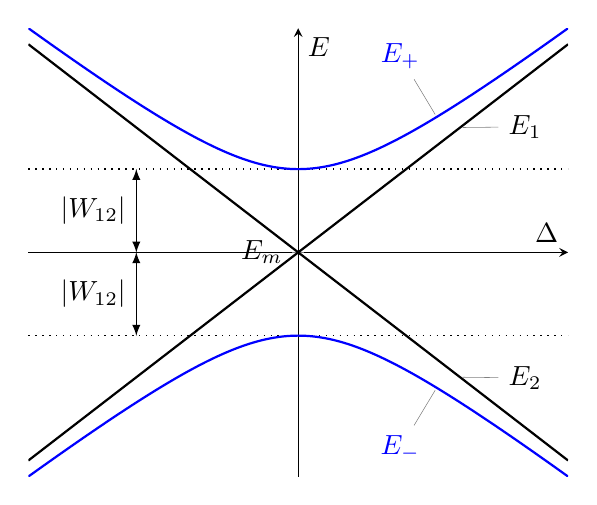
\begin{tikzpicture}
						\begin{axis}
						[
							axis x line=middle,
							axis y line=middle,
							samples=100,
							xlabel=$\Delta$,
							ylabel = $E$,
							ytick = {-1,1},
							yticklabels={,},
							ymajorgrids,
							major y grid style = {line width = 0.5pt,dotted,black},
							xtick = \empty,
							extra y ticks = {1,0},
							extra y tick style = {
								grid=none, 
								yticklabels={,$E_m$},
								yticklabel style={
									yshift=0ex,
									anchor=east
								}
							}
						]
							\addplot[mark=none, thick, smooth] expression { 0.5*x } node [pos=0.8,pin={1:$E_1$},inner sep=0pt] {}; 
							\addplot[mark=none, thick, smooth] expression { -0.5*x } node [pos=0.8,pin={-1:$E_2$},inner sep=0pt] {}; 
							\addplot[mark=none, thick, smooth, color=blue] expression { sqrt(1+(0.5*x)^2)} node [pos=0.75,pin={100:$E_+$},inner sep=0pt] {};
							\addplot[mark=none, thick, smooth, color=blue] expression { -1*sqrt(1+(0.5*x)^2) } node [pos=0.75,pin={-100:$E_-$},inner sep=0pt] {};
							\node (source) at (axis cs:-3,-0.12){};
							\node (destination) at (axis cs:-3,1.12){};
							\draw[latex-latex](source)--(destination);
							\node at (axis cs:-3.8,0.5){$\left|W_{12}\right|$};
 
							\node (source) at (axis cs:-3,0.12){};
							\node (destination) at (axis cs:-3,-1.12){};
							\draw[latex-latex](source)--(destination);
							\node at (axis cs:-3.8,-0.5){$\left|W_{12}\right|$};

						\end{axis}
					\end{tikzpicture}
					\caption{``Anticrossing'' of energy levels}
					\label{fig:anticrossing}
				\end{center}
			\end{figure}
			%
			%

			As one can guess from \figref{anticrossing}, we get an asymptotic behaviour for $|\Delta| \gg |W_{12}|$. For this case, we can approximate the eigenenergies as follows:
			\begin{align}
				E_\pm \approx E_m \pm |\Delta| \left( 1+\frac{1}{2} \left| \frac{W_{12}}{\Delta}\right| ^2+\dots\right).
			\end{align}

			Let us now have a look at the angle $\theta=\arctan(|W_{12}|/\Delta)$ defined previously in \eqref{eq:parameters}. For two different limits, we obtain

			\begin{align}
				\theta \approx \left\{ \begin{array}{lcl} \pm \frac{\pi}{2} & \text{for} & |\Delta| \ll |W_{12}|\\
				0,\pi & \text{for} & |\Delta| \gg |W_{12}| \end{array} \right. 
			\end{align}
			and at $\Delta=0$, we get:
			\begin{align}
				\ket{\psi_\pm}=\frac{1}{\sqrt{2}}\left(\pm \eexp{-i{\varphi}/{2}}\ket{\varphi_1}+ \eexp{i{\varphi}/{2}}\ket{\varphi_2}\right).
			\end{align}
				\paragraph{Examples.} In \figref{twostate}, examples for two-state systems are shown. They can be described quantum-mechanically with a double-well box potential. The single states shown for each system in \figref{twostate} are \emph{not} the eigenstates. In fact, superpositions of the shown states are the eigenstates of the system.

					\begin{figure}
						%\resizebox{\textwidth}{!}{
						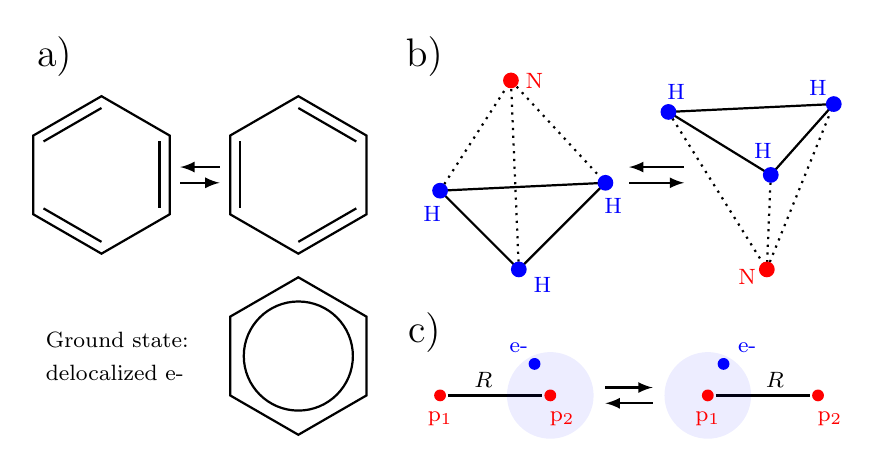
\begin{tikzpicture}

							%%benzene
							\node[align=left] at (-0.6,2.5) {\Large{a)}};
							%left benzene

							\draw[thick] (0 ,0) -- (-{sin(60)} ,{cos(60)}) -- (-{sin(60)} ,{cos(60)+1}) -- (0,{2*cos(60)+1}) -- ({sin(60)} ,{cos(60)+1}) -- ({sin(60)} ,{cos(60)}) -- cycle;

							\draw[thick] (0 , 0.15) -- ({-0.85*sin(60)} ,{0.85*cos(60)+0.15)});

							\draw[thick](-{0.85*sin(60)} ,{1.15*cos(60)+1-0.15}) -- (0,{2*cos(60)+1-0.15});

							\draw[thick] ({sin(60)-0.15*sin(60)} ,{0.85*cos(60)+1}) -- ({sin(60)-0.15*sin(60)} ,{1.15*cos(60)});


							%right benzene

							\draw[thick] (2.5 ,0) -- ({2.5-sin(60)} ,{cos(60)}) -- ({2.5-sin(60)} ,{cos(60)+1}) -- (2.5,{2*cos(60)+1}) -- ({2.5+sin(60)} ,{cos(60)+1}) -- ({2.5+sin(60)} ,{cos(60)}) -- cycle;

							\draw[thick] (2.5,{2*cos(60)+1-0.15}) -- ({2.5+0.85*sin(60)} ,{0.85*cos(60)+1});

							\draw[thick] ({2.5+0.85*sin(60)} ,{0.85*cos(60)+0.15}) -- (2.5 ,0.15);

							\draw[thick] ({2.5-sin(60)+0.15*sin(60)} ,{0.85*cos(60)+1}) -- ({2.5-sin(60)+0.15*sin(60)} ,{1.15*cos(60)});

							%\draw (-{sin(60)} ,{cos(60)}) -- ({sin(60)} ,{cos(60)+1});
							%\draw (-{sin(60)} ,{cos(60)+1}) -- ({sin(60)} ,{cos(60)});
							%\draw (0 ,0) -- (0,{2*cos(60)+1});

							%arrows between the two benzene states

							\draw[-latex,thick](1,{cos(60)+0.4})--(1.5,{cos(60)+0.4});
							\draw[latex-,thick](1,{cos(60)+0.6})--(1.5,{cos(60)+0.6});


							%ground state benzene

							\draw[thick] (2.5 ,-2.3) -- ({2.5-sin(60)} ,{cos(60)-2.3}) -- ({2.5-sin(60)} ,{cos(60)+1-2.3}) -- (2.5,{2*cos(60)+1-2.3}) -- ({2.5+sin(60)} ,{cos(60)+1-2.3}) -- ({2.5+sin(60)} ,{cos(60)-2.3}) -- cycle;

							\draw[thick] (2.5,{cos(60)-1.8}) circle ({0.8*sin(60)});

							\node[align=left] at (0.2,-1.3) {\footnotesize{Ground state:}\\ \footnotesize{delocalized \ch{e-}}};



							%%ammonia
							\node[align=left] at (4.1,2.5) {\Large{b)}};
							%ammonia up

							\draw[thick] (4.3,0.8) -- (5.3,-0.2)  -- (6.4,0.9) -- cycle;
							\draw[thick,dotted] (5.3,-0.2) -- (5.2,2.2);
							\draw[thick,dotted] (4.3,0.8) -- (5.2,2.2) -- (6.4,0.9);

							%\draw[thick] (4,0) -- (5,-1)  -- (6.1,0.1) -- (4.9,1.4) -- cycle;
							%\draw[thick] (5,-1) -- (4.9,1.4);
							%\draw[thick,dashed] (4,0) -- (6.1,0.1);
 
							\fill[fill=blue] (4.3,0.8) circle (0.1);
							\fill[fill=blue] (5.3,-0.2) circle (0.1);
							\fill[fill=blue] (6.4,0.9) circle (0.1);
							\fill[fill=red] (5.2,2.2) circle (0.1);
							\node[color=red] at (5.5,2.2) {\footnotesize{\ch{N}}};
							\node[color=blue] at (4.2,0.5) {\footnotesize{\ch{H}}};
							\node[color=blue] at (5.6,-0.4) {\footnotesize{\ch{H}}};
							\node[color=blue] at (6.5,0.6) {\footnotesize{\ch{H}}};

							%ammonia down

							\draw[thick] (7.2,1.8) -- (8.5,1) -- (9.3,1.9) -- cycle;
							\draw[thick,dotted] (8.5,1) -- (8.45,-0.2);
							\draw[thick,dotted] (7.2,1.8) -- (8.45,-0.2) -- (9.3,1.9); 

							%\draw[thick] (8,1) -- (9.3,0.2)  -- (10.1,1.1) -- (9.25,-1) -- cycle;
							%\draw[thick] (9.3,0.2) -- (9.25,-1);
							%\draw[thick,dashed] (8,1) -- (10.1,1.1);
 
							\fill[fill=blue] (7.2,1.8) circle (0.1);
							\fill[fill=blue] (8.5,1) circle (0.1);
							\fill[fill=blue] (9.3,1.9) circle (0.1);
							\fill[fill=red] (8.45,-0.2) circle (0.1);
							\node[color=red] at (8.2,-0.3) {\footnotesize{\ch{N}}};
							\node[color=blue] at (7.3,2.05) {\footnotesize{\ch{H}}};
							\node[color=blue] at (8.4,1.3) {\footnotesize{\ch{H}}};
							\node[color=blue] at (9.1,2.1) {\footnotesize{\ch{H}}};


							%arrows between ammonia states

							\draw[-latex,thick](6.7,{cos(60)+0.4})--(7.4,{cos(60)+0.4});
							\draw[latex-,thick](6.7,{cos(60)+0.6})--(7.4,{cos(60)+0.6});


							%% H2+ ion
							\node[align=left] at (4.1,-1) {\Large{c)}};
							%electron on right side
							\draw[thick] (4.4,-1.8) -- (5.6,-1.8);
							\fill[fill=blue, opacity=0.07] (5.7,-1.8) circle (0.55);
							\fill[fill=red] (4.3,-1.8) circle (0.075);
							\fill[fill=red] (5.7,-1.8) circle (0.075);
							\fill[fill=blue] (5.5,-1.4) circle (0.075);
							\node[align=right,color=red] at (4.3,-2.1) {\footnotesize{p$_1$}};
							\node[align=left,color=red] at (5.85,-2.1) {\footnotesize{p$_2$}};
							\node[align=right,color=blue] at (5.3,-1.2) {\footnotesize{\ch{e-}}};
							\node[align=right] at (4.85,-1.6) {\footnotesize{$R$}};

							%electron on left side
							\draw[thick] (7.8,-1.8) -- (9.0,-1.8);
							\fill[fill=blue, opacity=0.07] (7.7,-1.8) circle (0.55);
							\fill[fill=red] (7.7,-1.8) circle (0.075);
							\fill[fill=red] (9.1,-1.8) circle (0.075);
							\fill[fill=blue] (7.9,-1.4) circle (0.075);
							\node[align=right,color=red] at (7.7,-2.1) {\footnotesize{p$_1$}};
							\node[align=left,color=red] at (9.25,-2.1) {\footnotesize{p$_2$}};
							\node[align=left,color=blue] at (8.2,-1.2) {\footnotesize{\ch{e-}}};
							\node[align=left] at (8.55,-1.6) {\footnotesize{$R$}};

							%arrows between two electron configuration states
							\draw[-latex,thick](6.4,-1.7)--(7.0,-1.7);
							\draw[latex-,thick](6.4,-1.9)--(7.0,-1.9);
						\end{tikzpicture}
						%}
						\caption{Examples for two-state systems. a) Benzene: In the ground state, the electrons are delocalized. b) Ammonia (\ch{NH3}): The nitrogen atom is either found above or below the hydrogen triangle. The state changes when the nitrogen atom tunnels. c) Molecular ion \ch{H2+}: The electron is either localized near proton p$_1$ or proton p$_2$.}
						\label{fig:twostate}
					\end{figure}

					%\begin{itemize}
					%\item Benzene: Ground state: Delocalized electrons
					%\item Ammonia (\ch{NH3})
					%\item \ch{H2+}
					%\end{itemize}

		\subsection{Dynamical Aspects}
			\subsubsection{Time Evolution of $\ket{\psi(t)}$}
				After the static case we now want to investigate the dynamical properties of the two-state system. We calculate the time evolution of $\ket{\psi(t)} = \left(\begin{array}{cc} a_1(t) & a_2(t)\end{array}\right)^T$ with the Schrödinger equation and the perturbed Hamiltonian \eqref{eq:perturbedhamiltonian}:
				\begin{align}
					i\hbar \diff{}{t}\ket{\psi(t)}&=\left(\hat{H}+\hat{W}\right)\ket{\psi(t)},\\
					i\hbar \diff{}{t}\left(\begin{array}{c} a_1(t) \\ a_2(t) \end{array}\right) &= \left( \begin{array}{cc} \tilde{E}_1 & W_{12} \\ W_{12}^* & \tilde{E}_2 \end{array} \right) \left(\begin{array}{c} a_1(t) \\ a_2(t) \end{array} \right).
				\end{align}
				For the state $\ket{\psi(t)}$ we get
				\begin{align}
					\ket{\psi(t)}=\lambda \eexp{-i{E_+}t/{\hbar}} \ket{\psi_+} + \mu \eexp{-i{E_-}t/{\hbar}} \ket{\psi_-} \label{eq:psitimeevolution}
				\end{align}
				with the factors $\lambda$ and $\mu$.

				If we start in the state $\ket{\varphi_1}$, what is the probability
				\begin{align}
					P_2(t)=\left|\braket{\varphi_2|\psi(t)}\right|^2
				\end{align}
				to find the system in the state $\ket{\varphi_2}$? As a first step, we have to apply the initial condition to \eqref{eq:psitimeevolution} and express $\ket{\varphi}$ in terms of \eqref{eq:staticpsiplus} and \eqref{eq:staticpsiminus}:
				\begin{align}
					\ket{\psi(0)} \overset{!}{=}& \ket{\varphi_1}\\
											  = & \eexp{i{\varphi}/{2}} \left[ \cos\left( \frac{\theta}{2}\right) \ket{\psi_+}-\sin\left(\frac{\theta}{2}\right)\ket{\psi_-}\right]
				\end{align}
				By equating the coefficients we get for $\lambda$ and $\mu$:
				\begin{align}
					\lambda = \eexp{i{\varphi}/{2}}\cos\left(\frac{\theta}{2}\right), \qquad  \mu = -\eexp{i{\varphi}/{2}}\sin\left(\frac{\theta}{2}\right).
				\end{align}
				One thus gets:
				\begin{align}
					\hspace{-2mm} P_2(t)	=&\left|\braket{\varphi_2|\psi(t)}\right|^2 \\
											=& \left|\eexp{i\varphi} \sin\left(\frac{\theta}{2}\right)\cos\left(\frac{\theta}{2}\right)\left[\eexp{-i{E_+}t/{\hbar}} - \eexp{-i{E_-}t/{\hbar}}\right]\right|^2\\
											=& \sin^2(\theta)\sin^2\left(\frac{E_+-E_-}{2\hbar}t\right)
				\end{align}
				$P_2(t)$ can be expressed with $\Delta$ and $W_{12}$ alone. The obtained relation is called Rabi's formula:
				\begin{align}
					\Aboxed{P_2(t)=\frac{1}{1+\left(\frac{\Delta}{|W_{12}|}\right)^2}\sin^2\left(\sqrt{|W_{12}|^2+\Delta^2}\frac{t}{\hbar}\right)}
				\end{align}

				\begin{figure}
					\begin{center}
						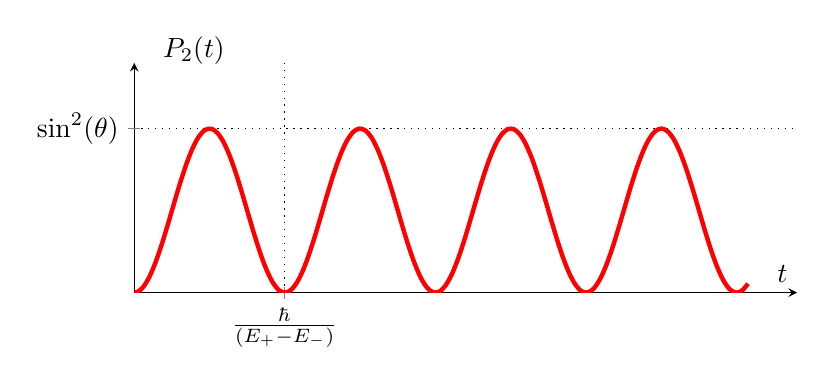
\begin{tikzpicture}
							\begin{axis}
							[
								axis x line=middle,
								axis y line=left,
								xmin = 0, xmax = {5.4},
								ymin = 0, ymax = {1.4},
								samples=200,
								xlabel=$t$,
								y label style={at={(axis description cs:0.09,.95)},rotate=-90,anchor=south},
								ylabel = $P_2(t)$,
								xtick = \empty,
								ytick = \empty,
								height = 4.5cm,
								width = 10cm,
								extra x ticks = {1.225},
								extra y ticks = {1},
								extra tick style={grid=major, grid style={line width = 0.5pt, dotted, black}},
								extra x tick labels={$\frac{\hbar}{(E_+-E_-)}$},
								extra y tick labels={$\sin^2(\theta)$},
							]
							\addplot[mark=none, ultra thick, smooth, color=red] expression {(sin(46.7*x*pi))^2};
							\end{axis}
						\end{tikzpicture}
						\caption{Rabi oscillations}
					\end{center}
				\end{figure}